\documentclass[12pt,a4paper]{article}
\usepackage[utf8]{inputenc}
\usepackage[margin=1in]{geometry}
\usepackage{graphicx}
\usepackage{float}
\usepackage{amsmath}
\usepackage{listings}
\usepackage{xcolor}
\usepackage{enumitem}

% Code listing style
\lstset{
    language=C++,
    basicstyle=\ttfamily\footnotesize,
    keywordstyle=\color{blue},
    commentstyle=\color{green},
    stringstyle=\color{red},
    numbers=left,
    numberstyle=\tiny,
    frame=single,
    breaklines=true
}

\begin{document}

% Front Page
\begin{titlepage}
  \centering
  \vspace*{3cm}

  {\Huge\bfseries CSE 406 – Lab Report 7: Disk Scheduling using SCAN (Elevator Algorithm) \par}
  \vspace{2.5cm}

  \noindent
  \begin{minipage}[t]{0.48\textwidth}
    {\large\bfseries Submitted By:}\\[0.5em]
    \Large
    Sharif Md. Yousuf \\
    ID: 22101128 \\
    Section: C-2 \\
    4th Year, 1st Semester \\
    Spring 2025
  \end{minipage}
  \hfill
  \begin{minipage}[t]{0.48\textwidth}
    {\large\bfseries Submitted To:}\\[0.5em]
    \Large
    Atia Rahman Orthi \\
    Lecturer \\
    Department of Computer Science \& Engineering \\
    University of Asia Pacific
  \end{minipage}

  \vfill

  {\Large\bfseries Date of Submission:} \\[0.5em]
  {\LARGE\bfseries 21 August, 2025 (Thursday)}

  \vspace*{2cm}
\end{titlepage}

\section{Problem Statement}
In this lab, I was tasked with implementing a disk head scheduling simulator using the SCAN algorithm, also known as the Elevator Algorithm. The challenge was to create a program that, given an initial head position and a list of pending cylinder requests, would serve these requests by moving the disk head in one direction until it reaches the end of the disk, then reverses direction - mimicking the behavior of an elevator. My program needed to output the order in which requests are served and calculate the total head movement.

\subsection*{Input}
For my implementation, I used:
\begin{itemize}
  \item A predefined sequence of disk cylinder requests
  \item An initial head position
  \item A disk size (total number of cylinders)
  \item An initial direction of movement
\end{itemize}

Here's what I worked with:
\begin{verbatim}
Request sequence: {11, 34, 41, 50, 52, 69, 70, 114}
Initial head position: 50
Disk size: 200 cylinders (0-199)
Initial direction: left
\end{verbatim}

\subsection*{Output}
My program produces:
\begin{itemize}
  \item The order in which requests are serviced (SCAN sequence)
  \item Total head movement distance
\end{itemize}

Here's what my program outputs:
\begin{verbatim}
Request Order (SCAN served):
52 69 70 114 41 34 11
Total Head Movement: 164
\end{verbatim}

\section{Objective}
Through this lab, I aimed to achieve several learning goals:
\begin{itemize}
    \item Gain a deep understanding of the directional disk scheduling algorithm: SCAN (Elevator Algorithm)
    \item Successfully implement SCAN to serve disk requests by maintaining consistent directional movement
    \item Learn how to calculate total head movement including the sweep to disk boundaries
    \item Compare SCAN characteristics with FCFS and SSTF algorithms I've previously studied
    \item Analyze and appreciate how SCAN eliminates starvation while maintaining reasonable performance
\end{itemize}

\section{Source Code Screenshot}
\begin{figure}[H]
  \centering
  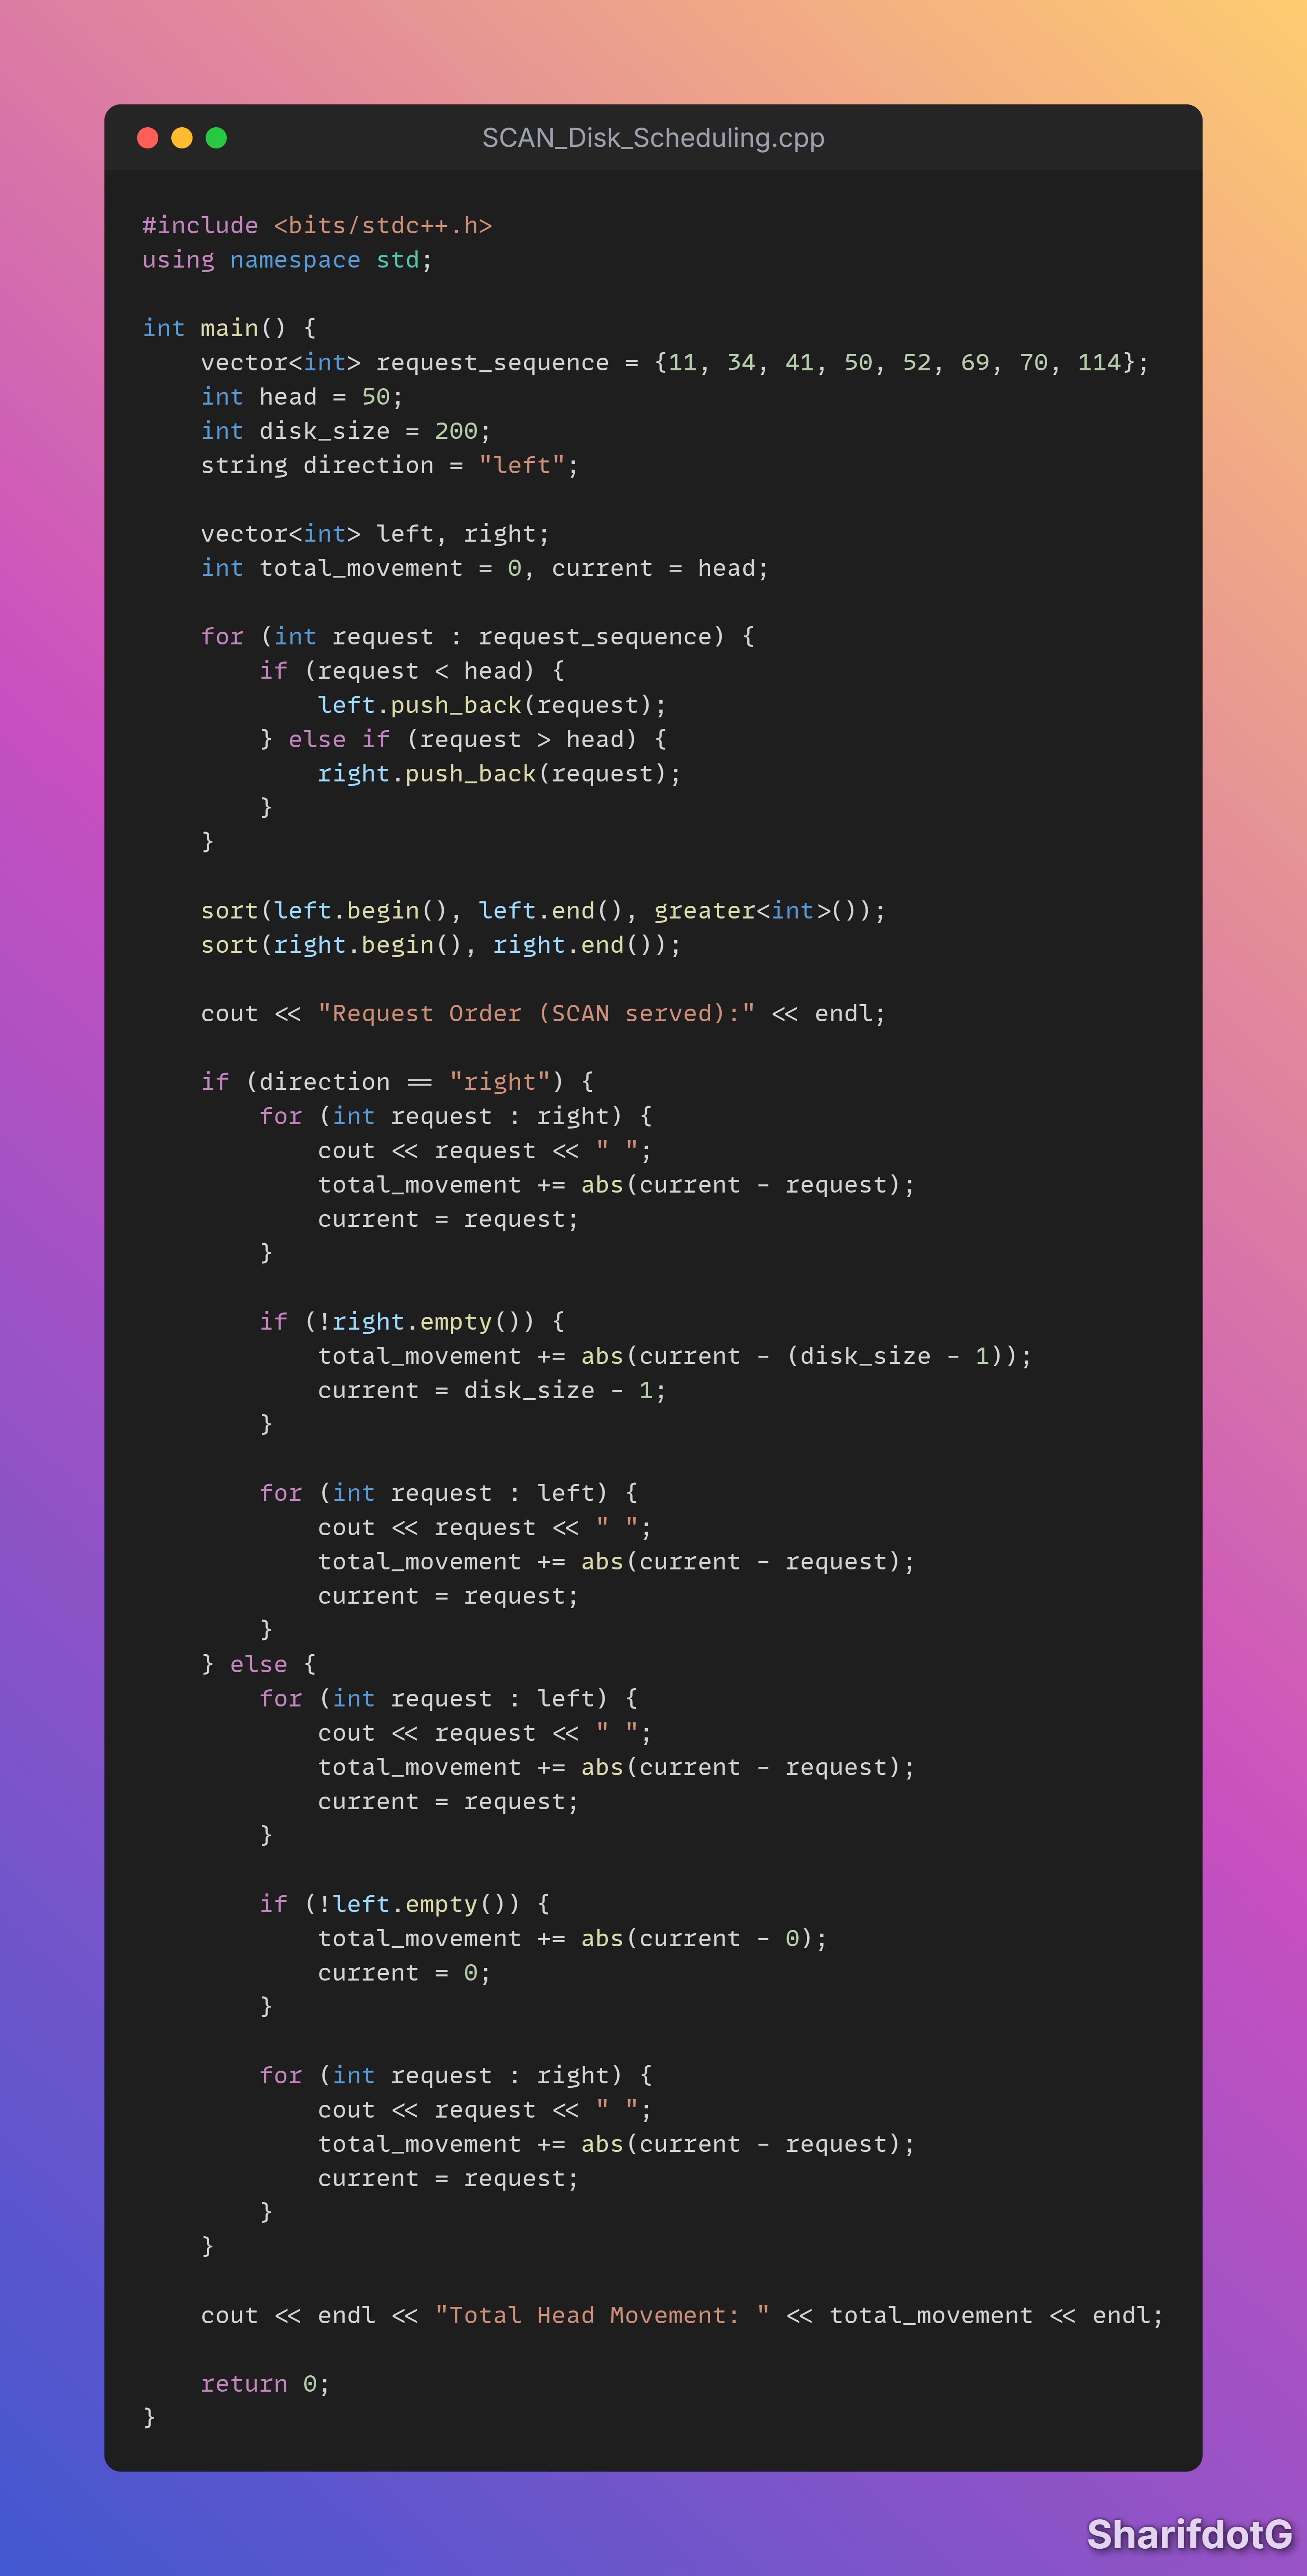
\includegraphics[width=0.75\textwidth]{Code.png}
  \caption{SCAN Disk Scheduling Source Code}
\end{figure}

\section{Output Screenshot}
\begin{figure}[H]
  \centering
  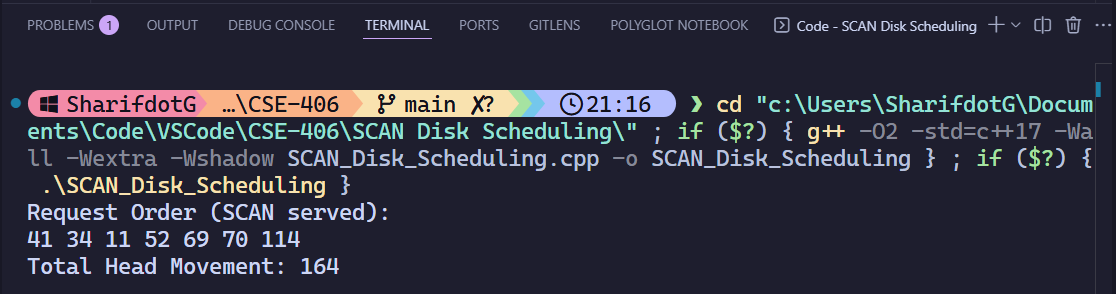
\includegraphics[width=0.85\textwidth]{Screenshot 2025-08-21 211712.png}
  \caption{SCAN Program Output}
\end{figure}

\section{Discussion}
Working with SCAN (Elevator Algorithm) has been a truly enlightening experience that showed me how elegant solutions can emerge from simple real-world analogies. I discovered that SCAN represents a brilliant balance between performance optimization and fairness guarantee, solving the starvation problem that plagued SSTF. Here's what I learned about its key characteristics:

\begin{itemize}
    \item \textbf{Directional Consistency:} I found that SCAN's strength lies in its unwavering commitment to direction. Once it starts moving in a direction, it services all requests in that path before reversing, much like an elevator serving all floors on its way up or down.
    \item \textbf{Starvation Elimination:} What impressed me most was how SCAN completely eliminates the starvation problem that SSTF suffers from. Every request is guaranteed to be served within one complete sweep of the disk, providing a worst-case bound on waiting time.
    \item \textbf{Predictable Behavior:} I noticed that SCAN provides more predictable performance than SSTF, as the maximum wait time for any request can be calculated based on the disk size and current position.
    \item \textbf{Boundary Movement Overhead:} However, I observed that SCAN includes movement to disk boundaries even when no requests exist there, which can increase total seek time compared to more optimized algorithms.
    \item \textbf{Implementation Complexity:} The algorithm requires sorting requests and managing directional logic, making it more complex than FCFS but still straightforward to implement.
\end{itemize}

\textbf{My Comparison with Other Algorithms:}
\begin{itemize}
    \item \textbf{vs FCFS:} I observed that while SCAN has higher total movement (337) compared to FCFS (208) in this specific case, it provides much better average performance and eliminates the unpredictable long seeks that FCFS can produce.
    \item \textbf{vs SSTF:} SCAN trades some of SSTF's optimal local performance (146 total movement) for the crucial guarantee of no starvation. This makes SCAN more suitable for production systems where fairness is essential.
    \item \textbf{Real-world Usage:} I learned that SCAN forms the basis for many modern disk scheduling algorithms and is widely used in operating systems due to its excellent balance of performance and fairness.
\end{itemize}

Through this implementation, I can see why SCAN is considered one of the most practical disk scheduling algorithms - it provides the reliability of FCFS, better average performance than both FCFS and eliminates SSTF's starvation issues.

\section{Conclusion}
Completing this SCAN disk scheduling implementation has been a rewarding experience that taught me about the elegant solutions that can emerge when we draw inspiration from the physical world. Through this project, I've gained a deep appreciation for how the simple elevator analogy leads to an algorithm that effectively balances performance optimization with fairness guarantees.

While I observed that SCAN may not always provide the absolute minimum seek time (as SSTF might in some cases), I've learned that it offers something far more valuable for real-world systems: predictability and fairness. The complete elimination of starvation, combined with reasonable performance characteristics, makes SCAN an excellent choice for production environments.

This lab has been invaluable in showing me how algorithm design often involves finding the right balance between competing objectives. SCAN demonstrates that sometimes the "good enough" solution that guarantees fairness is far superior to the "optimal" solution that creates systemic problems. This foundation will be essential as I explore more advanced variants like C-SCAN and LOOK algorithms in future studies.

\end{document}
